\chapter{Iteration 2}
\section{Planning}
This iteration goal was to allow students to post new submissions and view all previous submissions. Below is the list of stories and their assigned story points. The list is displayed in completion order.

\begin{itemize}
\item Add form to upload submission in student dashboard: 2 points
\item Display all previous submissions in student dashboard: 2 points
\end{itemize}

\section{Implementation}
\subsection{Adding the Student Upload Form}
A new route and template were created. This new page contained a form to upload a new submission as shown below in \autoref{fig:web-new-submission}. Only students can post new submissions, so this page is not accessible by staff. A title, module, and XML file are required. Uploading the XML file was a little more difficult due to the requirements. Following an online tutorial was sufficient enough to overcome this\cite{FlaskUploadingFiles}. The file that is submitted must be an XML file. This was checked in the HTML form, and in the Flask route function. The submitted XML file was parsed and the submission is inserted into the student submissions array in the database. A flash message was displayed upon success or failure as shown below in \autoref{fig:web-new-submission-success}.

\begin{figure}[H]
  \centering
  \fbox{
    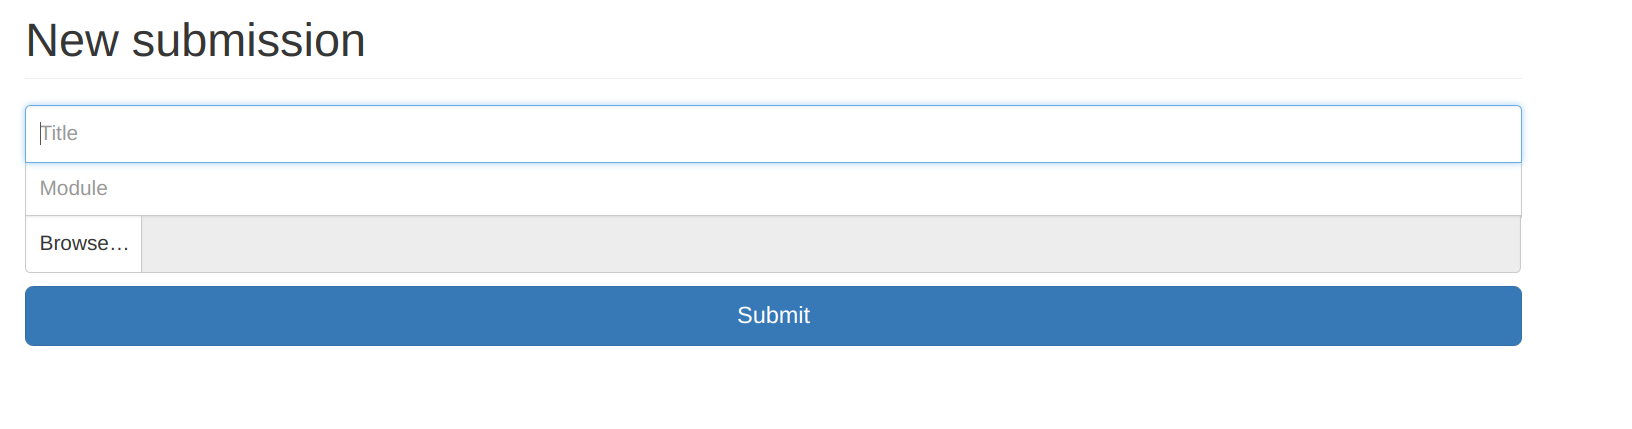
\includegraphics[height=\textheight,
    keepaspectratio=true,
    width=\textwidth,
    ]{figures/08-web-new-submission.png}
  }
  \caption[Web New Submission Page]{The submit page of the web-application. This is where students can submit their tracked data.}
  \label{fig:web-new-submission}
\end{figure}

\begin{figure}[H]
  \centering
  \fbox{
    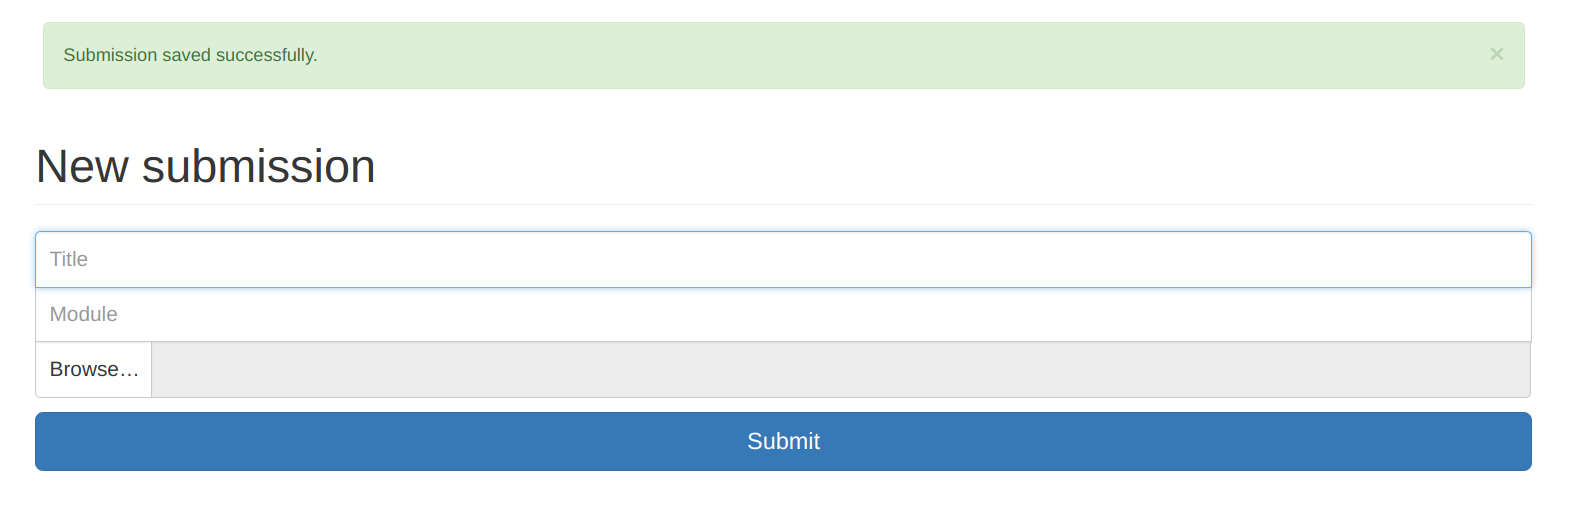
\includegraphics[height=\textheight,
    keepaspectratio=true,
    width=\textwidth,
    ]{figures/09-web-new-submission-success.png}
  }
  \caption[Web New Submission Success]{A success flash message is displayed when the form is successfully submitted and saved.}
  \label{fig:web-new-submission-success}
\end{figure}

\subsection{Displaying Previous Student Submissions}
The dashboard has been separated into two individual templates. One for staff and one for students. With functionality in place to post new submissions, these were now displayed to the user. Querying the database by filtering \texttt{uid}, the current students' submissions were retrieved. The submissions array was passed to the template to render. The template displays the submissions in a table as shown below in \autoref{fig:web-student-submissions}. The submissions were iterated, and each submission was added as a new table row. The submission title and module were displayed in the columns. More data for each submission may be added in future.

\begin{figure}[H]
  \centering
  \fbox{
    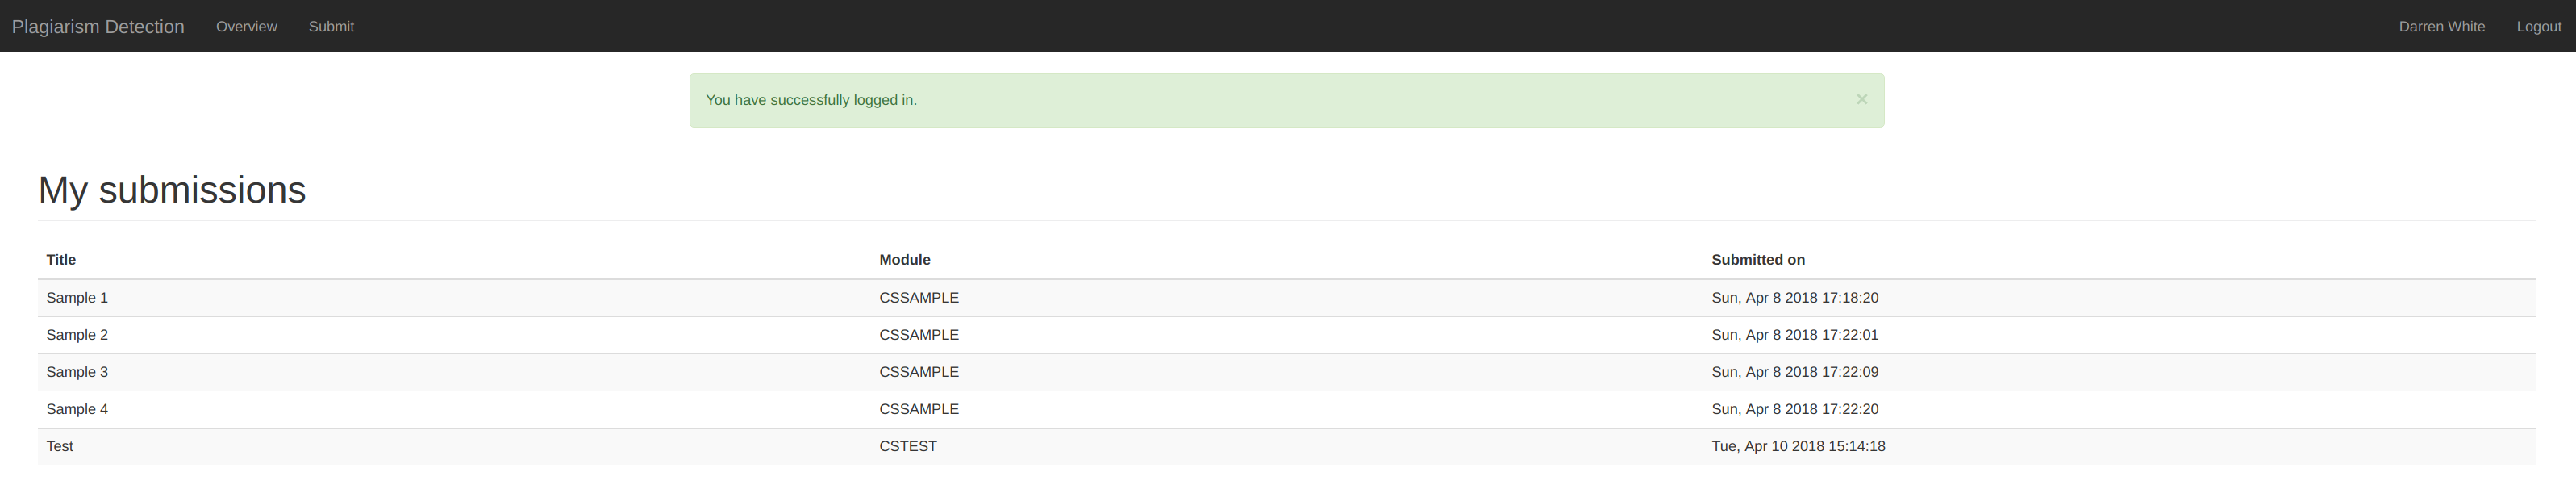
\includegraphics[height=\textheight,
    keepaspectratio=true,
    width=\textwidth,
    ]{figures/07-web-sign-in-success.png}
  }
  \caption[Web New Submission Page]{The dashboard page of the web-application for students. This is where students view their previous submissions. The flash message shown is only displayed after successfully signing in. Upon sign-in a redirect is sent to the dashboard.}
  \label{fig:web-student-submissions}
\end{figure}

\section{Retrospective}
This sprints' performance is extremely low in comparison to the first two. The sprint velocity is only 4. There were more stories initially for this sprint, but they were moved to the backlog and will be tackled in a future sprint. This was due to unforeseen health issues.
